\documentclass{article}

% Language setting
% Replace `english' with e.g. `spanish' to change the document language
\usepackage[english]{babel}

% Set page size and margins
% Replace `letterpaper' with `a4paper' for UK/EU standard size
\usepackage[letterpaper,top=2cm,bottom=2cm,left=3cm,right=3cm,marginparwidth=1.75cm]{geometry}

% Useful packages
\usepackage{amsmath}
\usepackage{amssymb}
\usepackage{graphicx}
\usepackage{braket}
\usepackage{stmaryrd}
\usepackage[colorlinks=true, allcolors=blue]{hyperref}
\usepackage{amsthm}
\usepackage{subcaption}
\usepackage{booktabs}
\usepackage{threeparttable}

\theoremstyle{definition}
\newtheorem{definition}{Definition}

\theoremstyle{plain}
\newtheorem{claim}{Claim}

\title{Learning Graph Invariants with PQCs}
\author{Jules DUPONT}

\begin{document}
\maketitle

\begin{abstract}
This document is a report for my project on the use of parametrised quantum circuits (PQCs) to learn graph invariants such as connectivity (QML, Topic 2), realized in the context of the Applied Quantum Algorithms course. It is structured as follows:
\end{abstract}

\section{Theory questions}

\begin{enumerate}
    \item For any $k\in \mathbb{N}^*$, we have:
    \begin{align*}
        h_k(M) &= \langle 0 | U_k | 0 \rangle \\
        &= \langle 0 | \Pi_{i=1}^k (W_i M) | 0 \rangle \\
        &= \langle 0 | W_kM \cdots W_1M | 0 \rangle \\
        &= \langle 0 | W_k\mathbb{I}M\mathbb{I} \cdots \mathbb{I}W_1\mathbb{I}M | 0 \rangle \\
        &= \sum_{j_1=0}^{N-1} \cdots \sum_{j_{2k-1}=0}^{N-1} \langle 0 | W_k | j_{2k-1} \rangle \langle j_{2k-1} | M | j_{2k-2} \rangle \cdots \langle j_2  | W_1 | j_1 \rangle \langle j_1 | M | 0 \rangle \\
        &= \sum_{j_1=0}^{N-1} \cdots \sum_{j_{2k-1}=0}^{N-1} w^{(k)}_{(0, \, j_{2k-1})} m_{(j_{2k-1}, \, j_{2k-2})}\cdots w^{(1)}_{(j_2, \, j_1)} m_{(j_1, \, 0)} \\
        \text{i.e.} \quad h_k(M) &= \sum_{j_1=0}^{N-1} \cdots \sum_{j_{2k-1}=0}^{N-1} m_{(j_{2k-1}, \, j_{2k-2})} \times \cdots \times m_{(j_1, \, 0)} \times w^{(1)}_{(j_2, \, j_1)} \times \cdots \times w^{(k)}_{(0, \, j_{2k-1})}
    \end{align*}
    If we flatten the index pairs into multi-indices with the mapping $m_{i_l} := m_{(j_{2k-2l+1}, \, j_{2k-2l})}$ for $ l = 1, \dots, k-1, $ and $ m_{i_k} := m_{(j_1, \, 0)}$ if $i_k < N$, $0$ otherwise, and denote $w^{(1)}_{i_1} \cdots w^{(k)}_{i_k}$ the coefficient that ultimately appears in front of the monomial $m_{i_1} \times \cdots \times m_{i_k}$, we obtain:
    \[ h_k(M) = \sum_{i_1=0}^{n-1} \cdots \sum_{i_{k}=0}^{n-1} m_{i_1} \times \cdots \times m_{i_k} \times w^{(1)}_{i_1} \cdots w^{(k)}_{i_k} \]
    which is a $k$-th degree multivariate polynomial of the entries of the matrix $M$.
    

    \item The formula involves $k$ many parameters sets, the $\mathbf{w}^{(j)}$, each of them containing $n$ entries. Therefore, there are exactly $n \times k$ parameters to set.
    
    Now, expanding the sums and using the commutativity of the multiplication we realize that many of the $m_{i_1} \times \cdots \times m_{i_k}$ terms are equal and can be grouped together. For example, with $k=2$, this is the case with $m_0 \times m_1$ and $m_1 \times m_0$. 
    Still, we have to determine a certain amount of coefficient products, precisely corresponding to the quantity of equations we are looking for. To explicit it, we shall count the number of effectively distinct words of the form $m_{i_1} \times \cdots \times m_{i_k}$, where the $i_j \in \{0, \dots, n-1\}$. 
    This can be viewed as a well-known combinatorial problem in which one has to place $k$ balls in $n$ boxes (each box may contain zero, one, or more than one ball). This is strictly equivalent to forming a word of length $k + (n-1)$ out of $k$ zeros intertwined with $n-1$ ones; one only needs to chose where to place the zeros and hence has $\binom{n+k-1}{k}$ possibilities. (Put differently, we have just recounted the number of multisets of size $k$ from $n$ elements.)

    All in all, there are $n \times k$ many parameters to set the coefficients $w_{i_l}^{(j)}$ while having $\binom{n+k-1}{k}$ many equations. We see numerically that, for large $n$,
    \[ \binom{n+k-1}{k} \gg nk \]
    meaning that we have much more equations to satisfy than we have parameters to play with. The model is emphatically not maximally expressive: it can only represent a strict subset of all $k$-th degree multivariate polynomials.

    \item 
    This is a crucial property, because


\end{enumerate}


\section{Implementation}

In this section, we report the implementation of the data generation step, the quantum model and the classical model.

\subsection{Dataset}

The data for our (quantum) machine learning problem was first generated following the data generation step described in the instructions. We generated $N$ random graphs using the Erdős–Rényi model, which builds graphs by choosing each of the possible edges with probability $p$. Using $\texttt{networkx}$'s function $\texttt{is\_connected(G)}$, connected graphs were given the label $0$, disconnected ones the label $1$. As we aimed to have a roughly equal number of connected and disconnected graphs, we varied the probability $p$ according to a uniform distribution roughly centered around the asymptotic threshold of $\frac{\ln n}{n}$ - where $n$ is the number of nodes.

Additionaly, as is standard in machine learning this dataset was divided into a training and a test datasets, according to a certain ratio $r$.

When choosing the size $N$ the full dataset should have, one should bear in mind the highly symmetrical nature of the problem: the property that we are trying to learn - connectivity - is invariant under nodes permutation, and the circuit ansätze we are going to use for the quantum model are equivariant under nodes permutation (see below). As such, it should be useless to have isomorph graphs - graphs that are equal up to a permutation of the nodes - in the training set: the training set should only consist of non-isomorphic graphs.

For reasonable values of the number of nodes $n$, these non-isomorphic graphs can be enumerated and counted: their count follows the sequence http://oeis.org/A000088. 

For example, for $n=5$, there are only of $34$ of them and the training set can just consist of these $34$ graphs.

However this count grows very fast: for $n=7$, there are already $1044$ of them. Rapidly, it becomes unreasonable to consider all the non-isomorphic graphs.

Consequently, we also implemented a data filtering procedure. It takes as input a training set of size $N_{\text{training}}$, removes all repetitions of isomorphic graphs, and outputs a filtered training set of size $N^{'}_{\text{training}}$.

In all cases, the test set was made of $N_{\text{test}}$ completely random graphs, where $N_{\text{test}}$ was chosen large enough to provide sufficient test metrics. The data filtering procedure described above was never applied to the test sets.

\subsection{Quantum model}

The quantum model consists of a standard Variational Quantum Algorithm (VQA) scheme: a Parametrized Quantum Circuit (PQC) was trained to learn the connectivity problem by minimizing a cost function with the help of a classical optimizer.

\subsubsection*{Parametrized Quantum Circuit}

The PQC was defined as suggested in the instructions as a sequence of $L$ layers of the form $W_iM$, where $W_j$ is a variational part and $M$ is a data encoding circuit block, and it was implemented using the open-source Python library Pennylane.

For the variational part, we first implemented the ansatz \[ W_i(\theta_i) = \otimes_{j=1}^n R_x(\theta_i) \] which consists of only one trainable parameter per layer (independently of the number of qubits $n$). The data encoding circuit block $M$ depends by definition on the encoded graph $G$, so we will subscript $M$ with the corresponding adjacency matrix $A$, i.e. write $M_A$. 

Before we show that the full circuit ansatz made of this simple variational ansatz $W_i(\theta_i)$ and that data encoding circuit block $M_A$ is permutation equivariant, let's redefine this property.

\begin{definition}[Permutation equivariance]
Let $U : \{0,1\}^{n \times n} \mapsto U(N)$ be a circuit ansatz parametrized by an adjacency matrix, and let $A$ be an arbitrary adjacency matrix.

We say that $U$ is \textit{permutation equivariant} if for all permutation matrices $P \in \mathcal{S}_{n \times n}$ and corresponding qubit permutation unitaries $\tilde{P}$ :
\[ U(PAP^T) = \tilde{P}U(A)\tilde{P}^{\dagger}\]
    
In other words, an ansatz that is defined by a graph is permutation equivariant if a permutation on the vertices of the graph results in the same ansatz to which we have correspondingly permutated the qubits: relabeling graph nodes and relabeling qubits are the same operation.
\end{definition}

\begin{claim} The circuit ansatz $U : A \rightarrow \Pi_{i=1}^L (W_i(\theta_i)M_A)$ is permutation equivariant. \end{claim}

\begin{proof}
For $P \in \mathcal{S}_{n \times n}$ an arbitrary permutation matrix, we have:
\[ M_{PAP^T} = e^{i\tilde{H}_G} = e^{i \tilde{P} H_G \tilde{P}^{\dagger}} = \tilde{P} e^{iH_G} \tilde{P}^{\dagger} = \tilde{P} M_A \tilde{P}^{\dagger} \]
where we used the fact that $\tilde{P}$ is unitary for the third equality. Additionally, $W_i(\theta_i)$ does not depend on the encoded graph, so we have:
\begin{align*}
U(PAP^{T}) &= \Pi_{i=1}^L (W_i(\theta_i) M_{PAP^T}) \\
&= \Pi_{i=1}^L (W_i(\theta_i) \tilde{P} M_A \tilde{P}^{\dagger}) \\
&= \tilde{P} \cdot \Pi_{i=1}^L (W_i(\theta_i) M_A) \cdot \tilde{P}^{\dagger} \\
\text{i.e. } U(PAP^{T}) &= \tilde{P}U(A)\tilde{P}^{\dagger}
\end{align*}
where we used for the third equality the facts that $\tilde{P}$ commutes with the $W_i$ and $\tilde{P}$ is unitary.

This shows that $U$ is permutation equivariant.
\end{proof}

With other variational ansätze such as \[ W_i^{'}(\theta_i^{(1)},\theta_i^{(2)}) = \bigotimes_{i=1}^n R_x(\theta_i^{(1)})R_y(\theta_i^{(2)}) \text{ and } W_i^{''}(\theta_i^{(1)},\theta_i^{(2)},\theta_i^{(3)}) = \bigotimes_{i=1}^n R_x(\theta_i^{(1)})R_y(\theta_i^{(2)})R_z(\theta_i^{(3)}), \] which were both implemented in the notebook and used in our experiments, or any other definition of the variational layers that does not depend on the encoded graph, the proof works exactly the same.

As a follow up, we allowed parametrization in the data encoding layers, that is rather use $M_{j,A} = e^{i\gamma_jH_G}$ where $\boldsymbol{\gamma}$ is a vector of trainable parameters. For we still have $M_{j, PAP^T} = \tilde{P} M_{j,A} \tilde{P}^{\dagger}$, the circuit ansatz remains permutation equivariant.

The output of this PQC was set to be the probability of observing the vaccum state $\ket{0}^{\otimes n}$, that is $\langle 0 | U_L | 0 \rangle$ - corresponding to the $k$-th degree multivariate polynomial $h_L(M)$ studied in the theory questions. Ultimately, after tuning the parameters, this probability would output a score predicting the likelihood of the graph encoded in the PQC being disconnected: after discretization around the threshold $0.5$, a value of $0$ would suggest a connected graph, $1$ for a disconnected graph.

\subsubsection*{Classical optimization loop}

Regarding the classical optimization loop, we defined our cost function as the mean over the Binary Cross-Entropy (BCE) losses between the PQC continuous prediction and the ground truth label over the entire training set. Then, we used a classical Adam optimizer to correspondingly vary the parameters.

This mean BCE loss was a key metric when assessing the training of a model, although another metric that was logged is the accuracy - defined as the proportion of correct predictions after discretization. Both these metrics were analyzed over the training data set and another test data set in order to evaluate the generalization capacity of the model. Each training was also evaluated by visually inspecting a confusion matrix, and in order to assess the convergence of the training of our models we visually inspected the loss curves.

Finally, the training of all models was logged under a separate \texttt{.jsonl} file, allowing for tracking of the evolution of key metrics such as the accuracies and making it easier to draw the plots presented in the next section.

\subsection{Classical model}

For the classical model, we made use of the \texttt{sklearn} library. Its built-in polynomial model \texttt{PolynomialFeatures} was pipelined with a \texttt{LogisticRegression}, applying the free weights $\mathbf{w}$ and appending a sigmoid for binary classification.

As for the quantum model a key metric that was used is the accuracy, evaluated on both the training and test sets.






.....


Should have started in the $\ket{+}^{\otimes n}$ state.

Create a non-equivariant ansatz and compare the number of layers required to achieve xx\% of accuracy.

p-test


\section{Results \& Discussions}

In this section we present some of the results that we obtained while training the quantum and classical models, and we try to answer the questions raised in the project instructions.

\subsection{First experiment}

In this first experiment we tried to learn the connectivity problem on graphs of size $n_{\text{num\_nodes}} = 8$ with our quantum model. We fixed the number of layers to $L=2$ but ran the experiment with the first and the second variational ansätze, namely $\bigotimes_{i=1}^n R_x(\theta_i)$ and $\bigotimes_{i=1}^n R_x(\theta_i^{(1)})R_y(\theta_i^{(2)})$. Regarding the used dataset, we generated $N=500$ random graphs - $247$ of which were connected - divided into a training set and a test set following a ratio $r = 0.2$, without any of the filtering mentioned earlier. We let the training run for $E=50$ epochs, allowed the parametrization of the data encoding layers (parameter $\boldsymbol{\gamma}$) and used an initial learning rate for the optimizer of $l=0.1$.

\autoref{fig:exp1_loss} shows the evolution of the cost function value (mean BCE loss) and the train and test accuracies over the training of the quantum model.

\begin{figure}[h]
    \centering
    \begin{subfigure}[b]{0.6\textwidth}
        \centering
        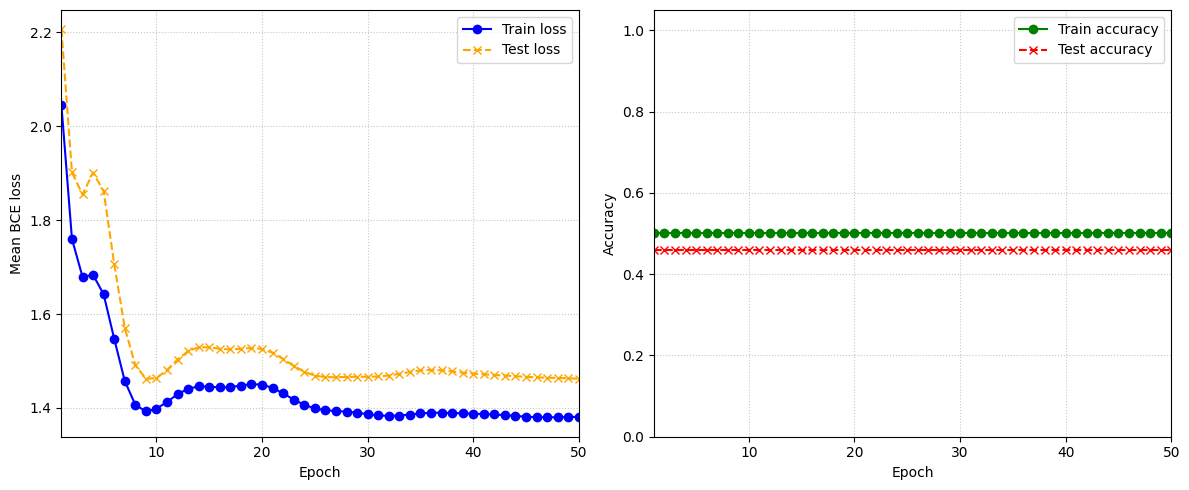
\includegraphics[width=\textwidth]{plots/report1.png}
        \caption{}
        \label{fig:exp1_loss}
    \end{subfigure}
    \hfill
    \begin{subfigure}[b]{0.35\textwidth}
        \centering
        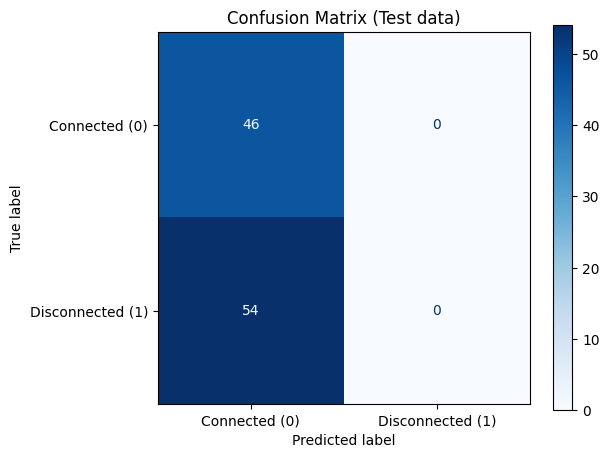
\includegraphics[width=\textwidth]{plots/conf1.png}
        \caption{}
        \label{fig:exp1_conf}
    \end{subfigure}
    \caption{(a) Evolution of the mean BCE loss, (b) accuracy throughout training, and (c) confusion matrix on the test data, for the quantum model with the first variational ansatz. See text for hyperparameter values.}
\end{figure}

Although the cost function globally decreases throughout the training, we see that the model completely fails at learning the connectivity problem as the accuracy on both the training and test sets remains constant around $50\%$ (and both sets contain roughly as many connected and disconnected graphs).

This is confirmed by the inspection of the confusion matrix represented in \autoref{fig:exp1_conf}: all graphs are classified as connected.

\autoref{fig:exp2_loss} shows the same curves, now using the second variational ansatz.

\begin{figure}[h]
    \centering
    \begin{subfigure}[b]{0.6\textwidth}
        \centering
        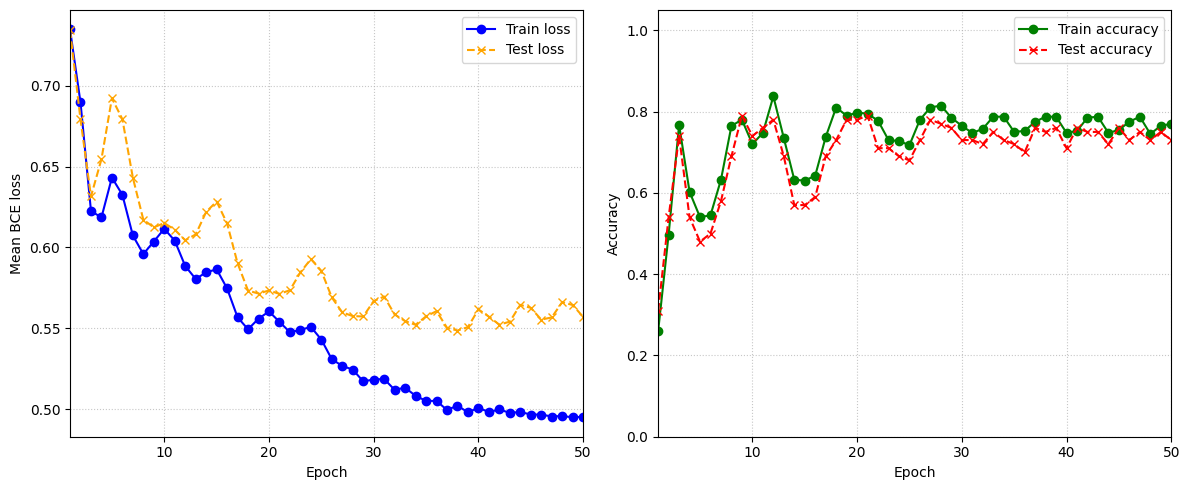
\includegraphics[width=\textwidth]{plots/report2.png}
        \caption{}
        \label{fig:exp2_loss}
    \end{subfigure}
    \hfill
    \begin{subfigure}[b]{0.35\textwidth}
        \centering
        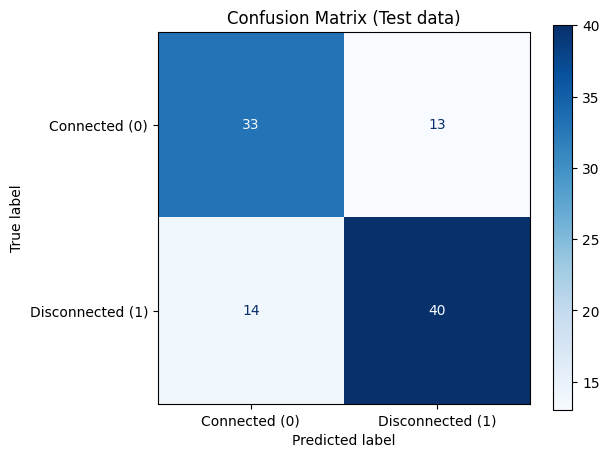
\includegraphics[width=\textwidth]{plots/conf2.png}
        \caption{}
        \label{fig:exp2_conf}
    \end{subfigure}
    \caption{(a) Evolution of the mean BCE loss, (b) accuracy throughout training, and (c) confusion matrix on the test data, for the quantum model with the second variational ansatz. See text for hyperparameter values.}
\end{figure}

The quantum model is now better at learning the connectivity problem: an accuracy of $\sim 73\%$ over the test set is reached. Observe the oscillations in the train and test accuracies, a phenomenon that will be discussed later.

The performance improvement is confirmed by the confusion matrix represented in \autoref{fig:exp2_conf}, which is more diagonal than earlier.

\subsection{Number of reuploading layers and variational ansatz}

In this other experiment, which mainly aimed at answering question e- from the project instructions, we trained the quantum model for the two first variational ansätze and for different numbers of reuploading layers (from $L=1$ to $L=5$).\footnote{all performance metrics of interest were averaged by training the model for all (number of re-uploading layers, variational ansatz) over 5 different random seeds (2 for $(L = 4, 1 \text{param/layer})$ and $(L = 5, 1 \text{param/layer})$).}

We again worked with graphs of size $n_{\text{num\_nodes}} = 8$, data sets of initial size $N=500$ but now applying the aforementionned data filtering procedure on the training set (effect discussed later). We always let the training run for $E=50$ epochs, allowed the parametrization of the data encoding layers and used an initial learning rate for the optimizer of $l=0.1$.

In \autoref{fig:accuracy_layers}, we plot the evolution of the final test accuracy (i.e. the accuracy over the test set, evaluated after the training) against the number of re-uploading layers for both variational ansätze.

We see that with the first variational ansatz, the quantum model consistently fails to learn the connecitivity problem (final test accuracies $\sim 50\%$).\footnote{although we want to note that during the experiments in other contexts we came across sets of hyperparameters where the model with the first variational ansatz did somehow manage to learn the connectivity problem.} With the second variational ansatz though, the quantum model achieves satisfying classification performances. For $L=1$, this is not very clear and the performance is rather widespread across the runs. But as of $L=2$, the reached final test accuracy is relatively high and stable ($75\% \pm 2\%$). As we continue increasing $L$, the final test accuracy does not continue increasing though.

However, \autoref{fig:time_layers} clearly shows how the resource consumption (expressed through the average time per epoch) of the training scales more rapidly with $L$ when the second variational layer is used. Indeed, the circuit ansatz that uses the second variational layer requires the training of $L$ more parameters than the one that uses the first variational layer.

\begin{figure}[h]
    \centering
    
\includegraphics[width=0.75\textwidth]{plots/test_acc.pdf}
    
    \caption{Final test accuracy against the number of re-uploading layers $L$. See text for hyperparameter values.}
    \label{fig:accuracy_layers}
\end{figure}

\begin{figure}[h]
    \centering
    
\includegraphics[width=0.75\textwidth]{plots/time.pdf}
    
    \caption{Average time per epoch of the training (in seconds) against the number of re-uploading layers $L$. See text for hyperparameter values.}
    \label{fig:time_layers} 
\end{figure}

\subsection{Data filtering}

We conducted another experiment to evaluate the significance of data filtering. Still with $n_{\text{num\_nodes}} = 8$, we trained the quantum model (with $L=2$ layers, and the second variational ansatz) until it reached a test accuracy $> 75\%$ or $50$ epochs, for both the cases were the training set was filtered and not filtered.

\autoref{tab:performance_metrics} summarizes the results of this experiment, repeated over 10 runs.

When the training set is filtered, the training epochs end faster. This was expectable, since the model has then less data points to train on ($\sim -30\%$). Yet, the mean wall time to reach the threshold ($> 75 \%$ accuracy) does not benefit the same shrinkage on average. Indeed, interestingly the model takes on average more training epochs to reach threshold when the training set is filtered than when it is not. This indicates that although our circuit ansatz is equivariant and should understand that the connectivity problem is invariant under nodes permutation, augmenting the training set with isomorphic graphs does still have a positive impact on the training. 

\begin{table}[htbp]
\centering
\begin{threeparttable}
\caption{Training Performance Metrics for Filtered vs. Unfiltered Datasets}
\label{tab:performance_metrics}
\begin{tabular}{lcc}
\toprule
\textbf{Metric} & \textbf{Filtered} & \textbf{Unfiltered} \\
\midrule
Success rate\tnote{a} & 8/10 & 9/10 \\
Mean time per epoch (s)\tnote{b} & $21.5 \pm 0.5$ & $29.3 \pm 1.0$ \\
Mean wall time to threshold (s)\tnote{b} & $346.2 \pm 153.3$ & $377.9 \pm 260.0$ \\
Mean epoch reached threshold\tnote{b} & $16.0 \pm 6.9$ & $12.8 \pm 8.4$ \\
\bottomrule
\end{tabular}
\begin{tablenotes}\footnotesize
\item[a] 'Success' is defined as reaching $\ge 75\%$ test accuracy within 50 epochs.
\item[b] Failed runs (where the model did not reach $\ge 75\%$ test accuracy within 50 epochs) are excluded from the time and epoch means.
\end{tablenotes}
\end{threeparttable}
\end{table}



\subsection{Reuploading layers parametrization}

In all previous experiments, we allowed parametrization in the data encoding layers through an additional trainable parameter vector $\boldsymbol{\gamma}$ as it appeared crucial for the model to successfully learn the connectivity problem from first toy experiments. 

To be more rigorous, we conducted a paired sample t-test to statistically prove the significance of the data encoding layers parametrization. 

For that, we defined the two following hypotheses:
\begin{itemize}
    \item Null hypothesis ($\mathcal{H}_0$): Parameterizing the data encoding layers has no significant effect on the model's performance. The true mean difference in final test accuracy between the parameterized model and the fixed model is zero.
    \item Alternative hypothesis ($\mathcal{H}_A$): Parameterizing the data encoding block significantly improves the model's performance. The true mean difference is greater than zero.
\end{itemize}
From our observation, $\mathcal{H}_A$ should be true. In order to accept or reject $\mathcal{H}_0$, we conducted the following paired experiment:
for each trial $i$ from $1$ to $N=10$,
\begin{enumerate}
    \item Pick a random seed $s_i$. 
    \item Train a model with \texttt{quantum\_model.ipynb}, which allows parametrization in the data encoding layers, manually setting the random seed to $s_i$. Record the final test accuracy, call it $X_i$.
    \item Train a model with \texttt{unparam\_quantum\_model.ipynb}, which does not allow parametrization in the data encoding layers, again manually setting the random seed to $s_i$ and - crucially - keeping all the other hyperparameters the same. In particular, the dataset is expected to be the exact same and we stop after the same number of epochs. Record the final test accuracy, call it $Y_i$.
    \item Record the paired difference $d_i = Y_i - X_i$
\end{enumerate}

With the data obtained throughout these $N$ trials and using the \texttt{scipy.stats} library, we obtained a $t$-statistic of $6.4$ and a $p$-value of $p = 0.0001$ for rejecting the null hypothesis $\mathcal{H}_0$. This means that we can say with high confidence that parametrizing the data encoding layers significantly improves model performance and this confirms our earlier observation.\footnote{In fact the unparametrized model barely ever learned the connectivity problem, as $\mu_{\text{unparam}} = 0.53 \pm0.04$.}






\subsection{Oscillations}

It is interesting to observe how not only the losses but also the accuracies evolve by following oscillations, as in \autoref{fig:oscillations}. This is likely due to the periodicty of the $\theta \mapsto R_{n}(\theta)$ parametrized unitaries, but complicates the question of choosing when to stop the training. Also, we could have implemented an exponential learning rate decay, as was done in \cite{DBLP:journals/corr/abs-2112-05261}, in order to avoid these oscillations.

\begin{figure}[h]
    \centering
    
\includegraphics[width=0.60\textwidth]{plots/fledged_osc.png}
    
    \caption{Fledged oscillations in the training and test accuracies during the training of a quantum model. This happens after $\sim15$ epochs in spite of the losses appearing to converge.}
    \label{fig:oscillations}
\end{figure}

\subsection{Performance plateau}

\subsection{Performance on unseen graph isomorphisms}

The fact that the train and test accuracies always stayed relatively close during our trainings indicates that there is likely no overfitting. But how do the models perform on graph isomorphisms they have certainly not encountered during their training? This should tell more about the generalization capacity of the models. 

To answer this question, we implemented a \texttt{generate\_novel\_test\_set(train\_data, num\_nodes, num\_new\_graphs)} utility that generates \texttt{num\_new\_graphs} graphs that are isomorphic to no graph from the \texttt{train\_data} set. Then, we evaluated our models on these novel test sets by computing an accuracy.

\subsection{Comparison with the classical model}

As was discussed earlier, the chosen baseline for the classical model consisted of learning the adjacency matrix directly - and not the encoded matrix.

A first experiment consisted of comparing the learning of the connectivity problem for the quantum and classical models with the exact same dataset ($n_{\text{num\_nodes}} = 7$, $N = 500$, $r=0.2$, data filtering), averaging over 10 runs.

\autoref{tab:quantum_vs_classical} shows the results of this experiment. Although the training of the classical model is almost instantaneous compared to the training of the quantum model, the classical model appears to suffer from overfitting: it learns perfectly on the graphs from the training set, but the achieved test accuracy hardly beats the quantum model, indicating that it struggles to generalize.

\begin{table}[h]
\centering
\begin{tabular}{lcc}
\toprule
\textbf{Metric} & \textbf{Quantum model} & \textbf{Classical model} \\
\midrule
Train accuracy      & $0.752 \pm 0.036$ & $1.000 \pm 0.000$ \\
Test accuracy       & $0.744 \pm 0.092$ & $0.775 \pm 0.135$ \\
Total training time & $338$s & $<1$s \\
\bottomrule
\end{tabular}
\caption{Comparison of the quantum and classical models, averaged over 10 runs. Uncertainties represent one standard deviation across seeds.}
\label{tab:quantum_vs_classical}
\end{table}

\bibliographystyle{alpha}
\bibliography{sample}

\end{document}
